%
%  $Description: Author guidelines and sample document in LaTeX 2.09$
%
%  $Author: ienne $
%  $Date: 1995/09/15 15:20:59 $
%  $Revision: 1.4 $
%

\documentclass[times, 10pt,twocolumn]{article}
\usepackage{latex12}
\usepackage{times}
\usepackage{balance}
\usepackage{graphicx}
\usepackage{amsmath}
\usepackage{amssymb}
\usepackage{times}
\usepackage{xspace}
\usepackage{color}

%\documentstyle[times,art10,twocolumn,latex8]{article}

%-------------------------------------------------------------------------
% take the % away on next line to produce the final camera-ready version
\pagestyle{empty}
\makeatletter
\DeclareRobustCommand\onedot{\futurelet\@let@token\@onedot}
\def\@onedot{\ifx\@let@token.\else.\null\fi\xspace}

\def\eg{\emph{e.g}\onedot} \def\Eg{\emph{E.g}\onedot}
\def\ie{\emph{i.e}\onedot} \def\Ie{\emph{I.e}\onedot}
\def\cf{\emph{c.f}\onedot} \def\Cf{\emph{C.f}\onedot}
\def\etc{\emph{etc}\onedot} \def\vs{\emph{vs}\onedot}
\def\wrt{w.r.t\onedot} \def\dof{d.o.f\onedot}
\def\etal{\emph{et al}\onedot}
\makeatother
%-------------------------------------------------------------------------
\begin{document}

\title{A Hierarchical Model for Real-time Overlapping Car Detection}

\author{Author(s) Name(s)\\
\emph{Author Affiliation(s)}\\
\emph{E-mail}\\
% For a paper whose authors are all at the same institution,
% omit the following lines up until the closing ``}''.
% Additional authors and addresses can be added with ``\and'',
% just like the second author.
%\and
%Second Author\\
%Institution2\\
%First line of institution2 address\\ Second line of institution2 address\\
%SecondAuthor@institution2.com\\
}

\maketitle
\thispagestyle{empty}

\begin{abstract}
In this paper, we propose a hierarchical model for detecting cars with significant overlapping. The model is composed of two layers: car pair layer and single car layer. Nodes on single car layer is conditioned on the specific type of that in car pair layer, and  each node is represented by a deformable part based template. With labeled car pair images, the model can be learned sequentially by using latent-SVM at each layer. A cascade object detection algorithm is then proposed to detect these overlapping cars efficiently. Experiments on a self-collected dataset show that the proposed model gets better detection performance than the single car detectors and can run in real-time.
\end{abstract}



%-------------------------------------------------------------------------
\Section{Introduction}

Most object recognition methods recognize objects individually. However, in real applications, images of cars usually occlude each other, because they are in traffic, or parked together. By occlusion, salient image features observed in single car images, such as break lights or bumpers may no longer be visible. The missing features make single car models fail on detecting overlapping cars.

In this paper, we propose to detect those overlapping cars using a hierarchical object models for both car pairs and single cars, where each model is a deformable part based object model. As is shown on Fig.\ref{fig::model}, the hierarchy is composed of two layers. The root layer is composed of nodes as car pair models for different views and relative poses. Each node in root layer is then further associated with two single car models, which are elements in the single car layer.

Using the latent-SVM formulation, templates in the first layer can be learned from all input car pair images simultaneously, and these training images are also clustered into groups, each supporting the training of corresponding template. Each group of car pair images are further used to train two single car templates, which are the templates shown on the second layer of Fig.\ref{fig::model}.

With the model hierarchy, overlapping cars can be detected by first using root layer templates to propose candidate car pairs, their views and relative poses. Then the corresponding car templates are then applied onto the candidate region to detect individual overlapped cars. Single, un-occluded cars and other objects are then detected over the rest of images.

Most of the object recognition literature concentrates on single, un-occluded car images.


 Dalal and Triggs \cite{hog} introduced a discriminative detector. Felzenszwalb \etal \cite{DPM} improved the detector by used a star-structured deformable part-based model (DPM), which is now state-of-the-art benchmark. Zhu et al. [5] further improved the Felzenszwalb's object detector by constructed a 3-layer tree-structure model, the model was more flexible to occlusion and appearance variations.  For detect efficiency, Felzenszwalb et al. [3] used a cascade framework to speed up object detection by more than one order of magnitude with negligible decrease in detection accuracy on PASCAL 2007 and PASCAL 2009 datasets. Pedersoli et al. [6] used a coarse-to-fine approach to dramatically accelerate the speed of object detection with part based models. Though the part based model is considered as a robust top-down structure, it could only handle partially occlusion and appearance variations. While recent work by [7-10] tries to address the general problem of occluded object detection, their models are too complicated to solve our specific problem in real-time.


Our car detector is based on the deformable part based model by Felzenszwalb et.al, as each node in our hierarchy is a template trained by this model. Readers are encouraged to read \cite{DPM} a through understanding, however related details will be introduced when necessary.

%-------------------------------------------------------------------------
\Section{The Model Hierarchy}

\begin{figure}
\centering
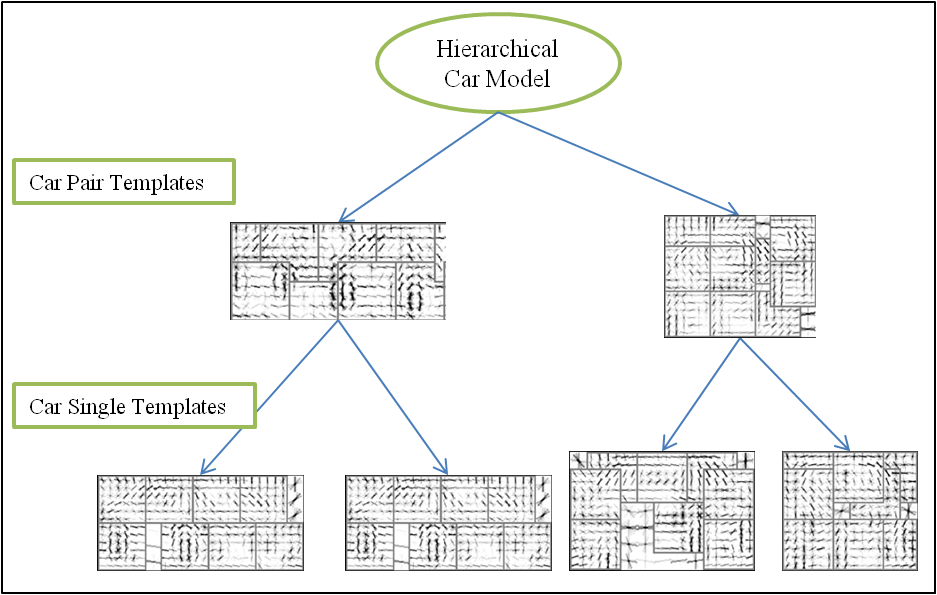
\includegraphics[width=3in]{./figs/fig1.png}
\caption{Examples of learned car pair templates and single car templates.}
\label{fig::model}
\end{figure}

Our proposed hierarchical model is based on following observation: although some significant single car features are unavailable, the overlapping cars distinguish themselves from un-occluded single cars and other objects by the repetition of remaining significant car features. This leads us to investigate the possibility of detecting these cars by first detecting groups of cars, where a car pair is the most basic and generic elements of groups.


Following this intuition, we propose a hierarchical model with two layers: car pair layer and occluded single car layer.

The first layer is composed of templates specifying different possible combinations of two cars. In our application, combinations are generally decided by two factors, the view of cars and their relative positions.  Each combination is then split into two nodes in the occluded car layer, and each one is a template of occluded car corresponding to the view and relative position of its parent car pair. 

Templates in each node is learned from deformable part based models (DPMs). Each DPM can be considered as a star-shaped graphical model consisting of a set of $p+1$ nodes $\{n_0, \cdots, n_p\}$; $n_0$ is called the root and the part nodes $\{n_1, \cdots , n_p\}$ are connected to the root. 

Score of such a template is composed of appearance terms and geometry terms. Appearance term is the inner product of a HOG \cite{hog} feature $\phi_p (x)$ at position x  with a discriminant $w_p^a$ for p. The location $x_p$ of each part p is allowed to deviate from the root location $x_0$, but is panelized by a quadratic cost as the geometry term:
\begin{equation}
w_p^g \psi(x)=w_p^g \cdot [(x_p-x_0 ),(x_p-x_0 )^2 ]
\end{equation}
Concatenating all terms, template score can be written as $\mathbf{w}\cdot \mathbf{f}(x)$, which is of the form:
\begin{eqnarray}
[w_0^a ,\cdots ,w_p^a ,w_p^g ] \cdot [\phi_0 (x), \cdots ,\phi_p (x) ,\psi_p (x)]
\end{eqnarray}

%-------------------------------------------------------------------------
\Section{Layered Model Training}

\begin{figure}
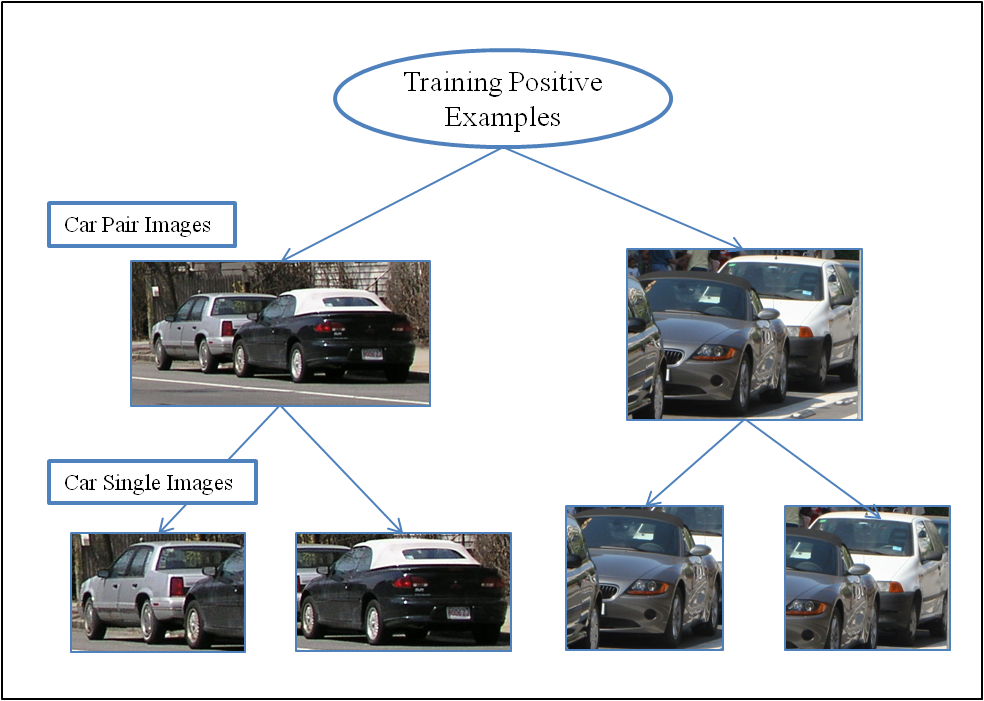
\includegraphics[width=3in, height =1.9in]{./figs/fig2.png}
\caption{Examples of training images for car pair templates and car single templates.}
\label{fig::data}
\end{figure}


We propose to learn these car templates in two batches. 

First, car pair templates are learned from labeled car pair images. We use the latent support vector machine (latent-SVM), which could learn a mixture of DPMs covering different types of car pair combinations, and at the same time cluster the training car pairs into corresponding combinations.  

The latent-SVM proposes to minimize the $l_2$ regularized loss over several DPMs. It is optimized by alternatively optimizing the template weights w for DPMs given fixed image clusters, and optimizing training image clusters by fixing the template weights. More details of the latent-SVM formulation and corresponding algorithm can be found in \cite{DPM}.  
Examples of the learned car pairs templates and car pair image clusters are shown in Fig.\ref{fig::model} and Fig.\ref{fig::data} correspondingly. We can clearly see different car pair combinations from these templates, and the car pair images are clustered accordingly. 

Given the car pair templates and training image clusters, training templates on single car layers are straightforward: for each cluster, we just crop the single car images from car pairs, and train two DPMs individually, each for one car in the car pair. Examples of these single car templates are shown in Fig.\ref{fig::data}.  


%-------------------------------------------------------------------------
\Section{Cascade Detection}

From training data, we learned \textcolor{red}{X} rough car pair combinations and \textcolor{red}{X}  single car templates. A naive detection method would apply these \textcolor{red}{XX}  templates over the whole image area, add car pair scores to its corresponding single car score and use non-maximum suppression to report windows of overlapped single cars. However, this naive implementation is impractical because it is impossible to run \textcolor{red}{XX}  templates in real time. Besides, we also need to detect un-occluded single cars and other objects such as pedestrians and motor-bikes. 

To satisfy the time budget, we propose to detect overlapped cars in cascade. We first run the \textcolor{red}{X}   car pair templates using the branch and bound method proposed in \cite{rapidDetection}, over the whole image area. By running non-maximum suppression jointly over the \textcolor{red}{X}   template score maps, we can propose a number of candidate car pair object bounding boxes, each with its car pair combination id.  We use a low template score threshold in the branch and bound, so as to make sure that all promising car pairs are detected.

For each proposed car pair bounding box, we enlarge it 1.5 times, and use the two single car templates with same car pair combination id to search for the two occluded cars in this region. If two car accept this proposal and report both car pair and the two car instances to our system. Otherwise, we reject this car pair bounding box. 

Compared with applying a template onto whole image, the time searching in a local bounding box area can be almost neglected. So, by this cascade, only \textcolor{red}{X}   instead of \textcolor{red}{XX}  car templates are used across the whole image area, roughly 2/3 of the computation times are saved. 

Our surveillance system targeted at street scenes, where overlapped car pairs appear much more frequently than single cars and other object categories. To save more computation, we propose to detect these overlapping cars first, and mask out these reported car pair bounding box areas in detecting single un-occluded cars and other objects.
Because of masking, branch and bound, and cascading, adding our car pair detection module did not increase the overall processing time of the whole system.


%-------------------------------------------------------------------------
\Section{Experiments}

To evaluate the performance of our proposed method, we collected 286 images from street view scenes. For each image, we labeled all the car pairs, overlapped single cars in the car pair, and other single cars in the image. Overall, we obtained 640 car pairs, 1280 overlapped single cars and 302 single cars. We used half of images for training, and the rest for testing.
In experiments, we compared our method with the following baseline methods:
\begin{enumerate}
\item we just use the overlapped single cars in the training images to train a deformable part based model. we call the model Baseline 1.
\item we use all single cars in the training images to train a deformable part based model. we call the model Baseline 2.
\end{enumerate}
We test all of the three model in our dataset and their average precision are as follows: Baseline 1: 0.525, Baseline2: 0.511, V4: 0.454. Baseline1 and Baseline2 are more robust to occlusion. 
The average precision curves are shown in Fig.\ref{fig::PRCurve}.

\begin{figure}
\centering
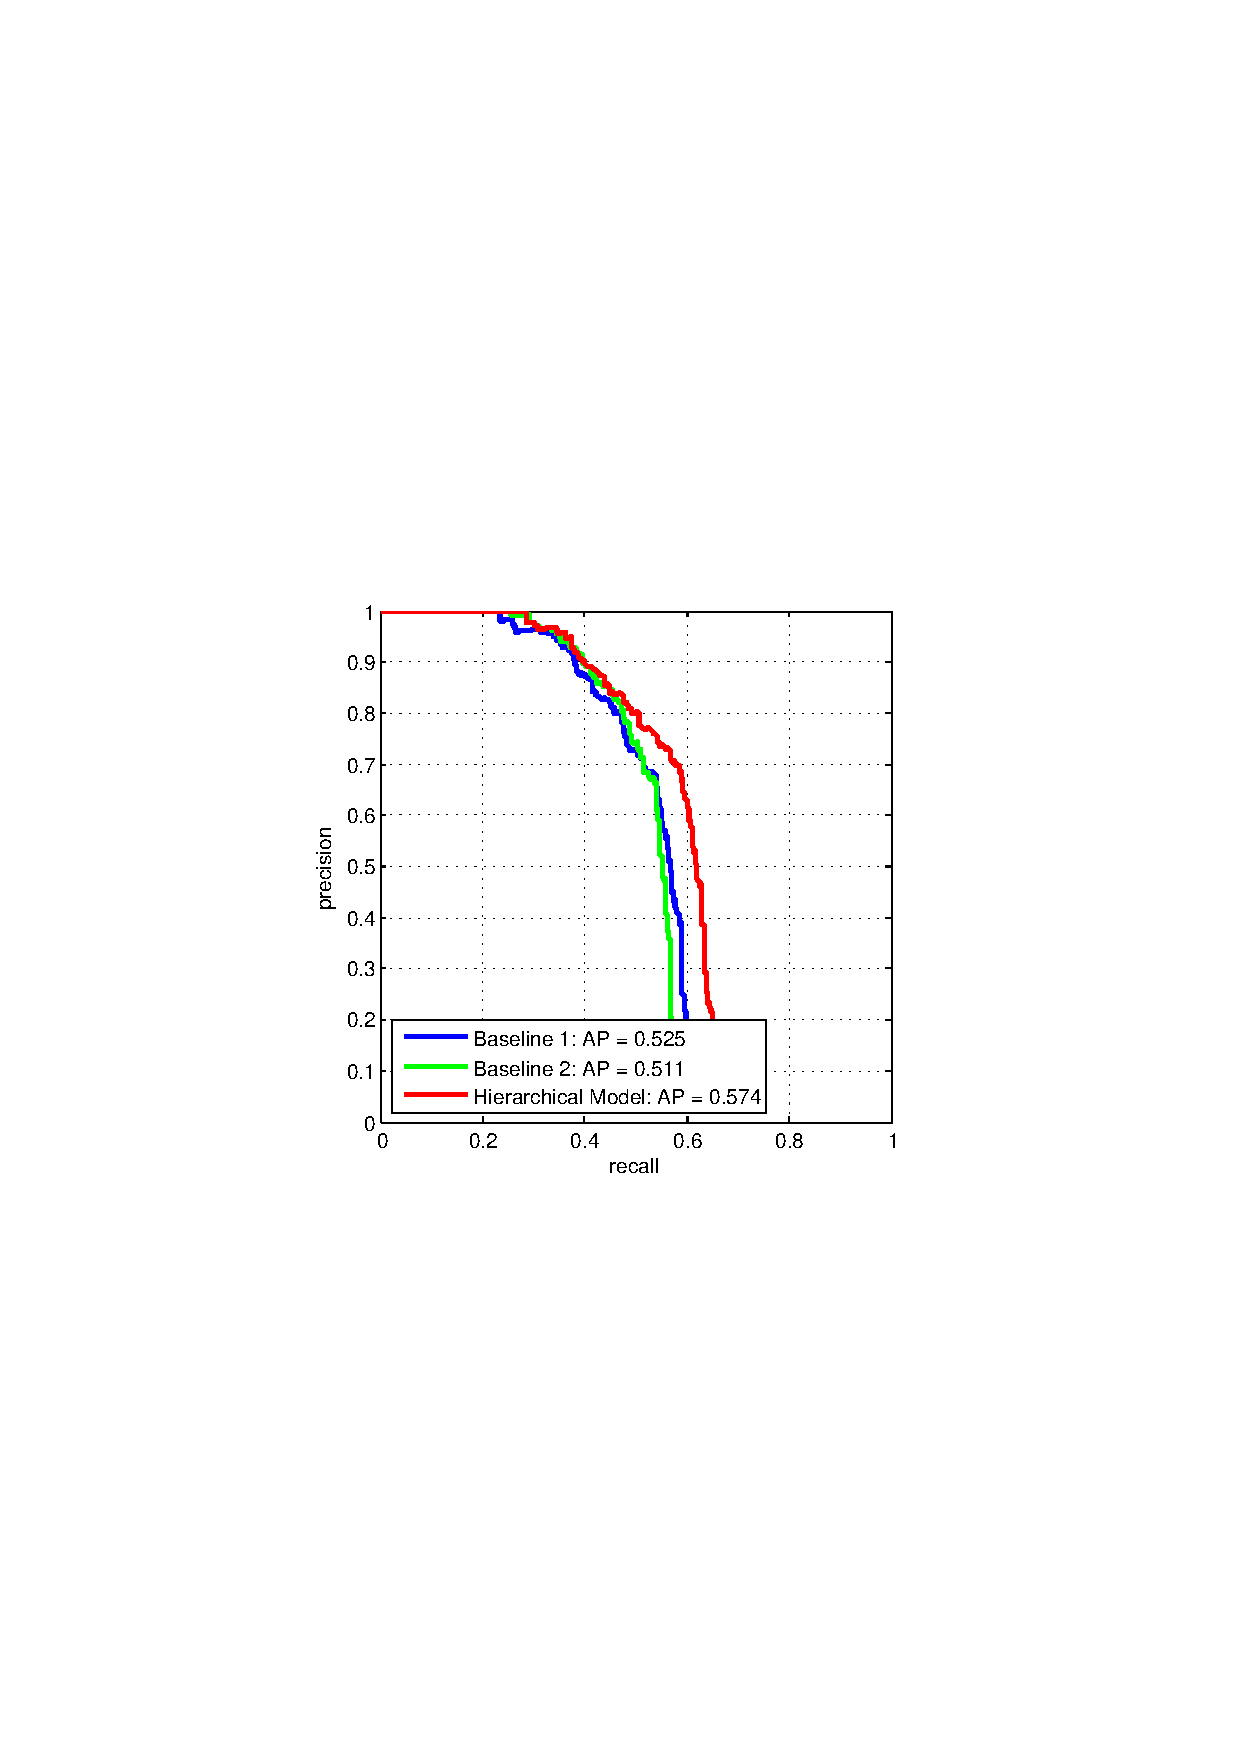
\includegraphics[width=3in, height =2.5in]{./figs/pr_comp.pdf}
\caption{Precision/Recall curves for Baseline 1, Baseline 2 and hierarchical model}
\label{fig::PRCurve}
\end{figure}
 


We evaluate the performance of these methods by using precision-recall curves, which are shown in Fig.3. From the curves, we can see that the use of hierarchical model can effectively improve the detection accuracy.

Fig.\ref{fig::sample} shows some outputs from our real surveillance systems, from the results, we can see that our proposed method can reliably detect these overlapped cars. As a comparison, we also show the results of our system without our car pair module, from which we can see that many cars are missed because some portions of them are occluded by cars before or behind them.


\begin{figure}
\centering
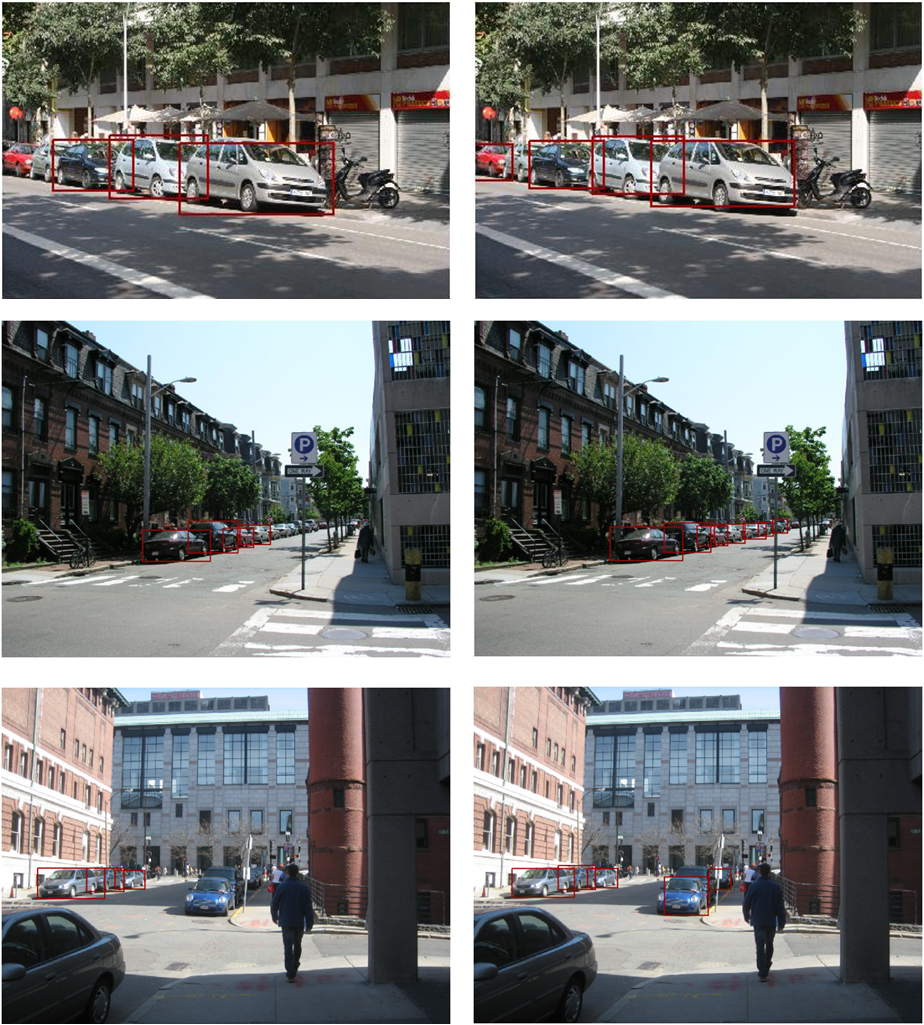
\includegraphics[width = 3in]{./figs/fig3.png}
(a) \hspace{1.2in}(b)
\caption{Detection result samples: (a) baseline 1;(b) ours.}
\label{fig::sample}
\end{figure}


%-------------------------------------------------------------------------
\nocite{ex1,ex2}
\bibliographystyle{latex12}
\bibliography{latex12}

\end{document}

